\subsection{Results} \label{unsupervised_approach_results}

Once we have the vector representations of documents and subjects, we can compute the cosine similarity between them to determine how similar they are regarding their semantic content. Due to the hierarchical nature of the subjects, we first compute the similarities of every document with the subjects of the first level, what we call fields, and then compute the similarities for the descendants of the five most similar fields for each subject. We then store the 50 most similar subjects.

However, we first have to choose how to compute the similarities between documents and subjects. The proper experiments with the methods are presented in chapter \ref{eval}. Here, we discuss some examples and perform a qualitative assessment of the three methods. We only consider fields to not compute so many similarities, as they are expensive.

\subsubsection{Word vector combination} \label{unsupervised_approach_results_combination}

\begin{figure}
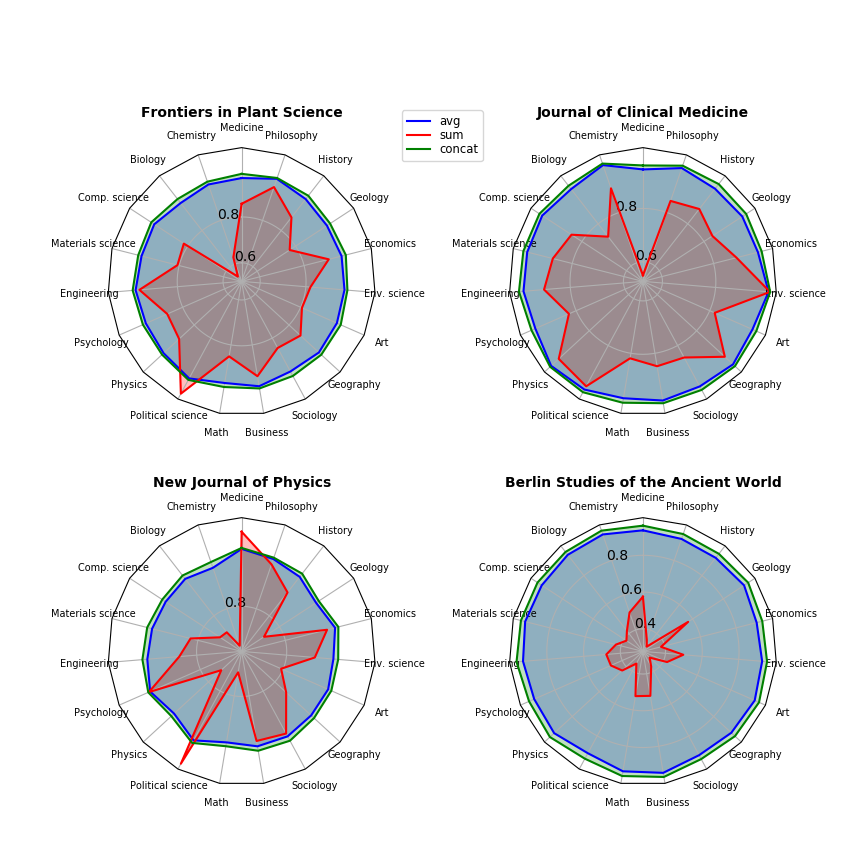
\includegraphics[width=\textwidth]{figures/unsupervised_approach/results/radar charts.png}
  \caption{Distances between venues and fields, for the three distance metrics.}
  \label{fig:combination_distance}
\end{figure}

In figure \ref{fig:combination_distance}, we show the results of the three methods for four venues, each belonging to a different field. The distances shown are the average distances of the documents that belong to each of the venues. In the upper left corner, the average distances of the documents that were published in \textit{Frontiers in Plant Science} are shown, which belongs to the field of \textit{Biology}. All three methods successfully identified the correct field on average.

The \textit{sum} method has the most expressive results. It assigns the documents \textit{Chemistry} in second place, and the distance between \textit{Biology} and \textit{Chemistry} exceeds $0.1$. On the other two methods, all three top options differ by around $0.01$. In fact, in the figures, one can see that the average distances of the concatenation and averaging methods are always around $0.95$. The difference between them occurs at a much lower scale. This shouldn't be a problem, as the distances can be rescaled afterwards.

All three methods also identified correctly the field of the venue \textit{Journal of Clinical Medicine}, shown in the upper right corner of figure \ref{fig:combination_distance}. Even for the averaging and concatenation methods, it is clear to see the smaller distance for the \textit{Medicine} field.

In the lower left corner, the average distances for the publications of \textit{New journal of Physics} are shown. None of the three methods places \textit{Physics} among their top three fields. The averaging and sum methods guess \textit{Chemistry} as the top field, whereas the concatenation method guesses \textit{Geology}. Physics is expected to be harder to guess because of its ubiquitous impact. It is closely related to other fields, mainly because it can be applied to any natural science.

The average distances between the fields and the documents published in \textit{Berlin Studies of the Ancient World}, which encompasses research in the fields of \textit{History} and \textit{Philosophy}, are shown in the lower left corner. The sum method was the only one to include both fields in their top three guesses, with \textit{Geography} between them. The other two methods guessed \textit{Political Science}, \textit{Economics} and \textit{Sociology}. Although similar, these were not the correct fields.